\documentclass[12pt]{article}
\pagestyle{empty}
\usepackage{amsmath, amssymb, amsthm}
\usepackage{latexsym, epsfig, ulem, cancel, multicol, hyperref}
\usepackage{graphicx, tikz, subfigure,pgfplots}
\usepackage[margin=1in]{geometry}
\setlength{\parindent}{0pt}
\usepackage{multirow}
\usepackage{mathtools}


\newcommand{\R}{\mathbb{R}}
\newcommand{\dydx}{\frac{dy}{dx}}
\usepackage{verbatim}
\usepackage{tikz}
\usepackage{pgfplots}

\newcommand{\wsnumber}{1}
\newcommand{\wstopic}{Vectors}
\pgfplotsset{
    every linear axis/.append style={
       axis x line=center,
       axis y line=center,
       xlabel={$x$},
       ylabel={$y$}
    },
    every axis plot/.append style={thick,mark=none}
}
\tikzset{
    point/.style={circle,draw,fill,minimum width=0.3ex,inner sep=0pt,outer sep=0pt},
    every label/.append style={black}
}


\usepackage[margin=1in]{geometry}
\usepackage{amsmath, amssymb, amsthm, graphicx, hyperref}
\usepackage{enumerate}
\usepackage{fancyhdr}
\usepackage{multirow, multicol}
\usepackage{tikz}
\pagestyle{fancy}
\fancyhead[RO]{Dennis Li}
\fancyhead[LO]{MA-UY 3113 Complex Variables and Linear Algebra }
\usepackage{comment}
\newif\ifshow
\showfalse

\ifshow
  \newenvironment{solution}{\textbf{Solution.}}{}
\else
  \excludecomment{solution}
\fi

\renewcommand{\thefootnote}{\fnsymbol{footnote}}
\usepackage{comment}


\newtheorem*{remark}{Remark}


\begin{document}

\begin{center}
\ifshow
  \textbf{\Large Homework 4 Solution}\\
\else
  \textbf{\Large Homework 4}\\
\fi
Due: Friday March, 15 , by 11:59pm,\\via Gradescope\\
\end{center}

\hrule

\vspace{0.2cm}

\begin{enumerate}[$\bullet$]
\item  {\textbf{\textit{Note that you must assign a page to each problem you submit.}}}   Gradescope has great YouTube videos available on how to submit homework.  \textit{\textbf{Failure to submit homework correctly will result in a zero on homework.}}
\item Problems that appear with the notation \colorbox{yellow}{$\ast$} will require you to TeX your solution.  If no highlighted star appears, then a hand written solution is OK.  
\item Late homework is not accepted.  Lateness due to technical issues will not be excused.  
\end{enumerate}

\hrule

\vspace{0.5cm}




\begin{enumerate}


\item  \colorbox{yellow}{$\ast$} Let $f(z) = u(z) + iv(z)$ be analytic in a region $D$.  Use the Cauchy-Riemann equations to show that $f'(z)$ is also analytic in $D$.  \\
\textbf{Solution:}\[
\text{$f(z)=u(z)+iv(z)$ is analytic in D}
\]
\[
\therefore \text{by Cauchy Riemann Equation } f'(z)=u_x +iv_x
\]\[
\text{and } u_x=v_y
\]\[
u_y=-v_x
\]
now examine $f''(z)$ we can do the following.
\[
\frac{\partial}{\partial x} (u_x=v_y)
\]
\[
\frac{\partial}{\partial y} (u_y=-v_x)
\]
if this relationship holds, we can determine that $f'(z)$ is also analytic in D
\[
u_{xx}=v_{yx}
\]\[
u_{yy}=-v_{xy}
\]
adding the first equation to the second we can obtain
\[
u_{xx}+u_{yy}=v_{yx}-v_{xy}
\]
cleaning it up, we have 
\[
u_{xx}+u_{yy}=v_{yx}-v_{xy}
\]
since $f(z)$ is analytic in $D$, we can deduce that $u(x,y)$ and $v(x,y)$ are continuous and differentiable
\[
 v_{yx}=v_{xy}
\]
\[
u_{xx}+u_{yy}=\nabla^2u=0
\]
we can now see that the following equation holds
\[
u_{xx}+u_{yy}=v_{yx}-v_{xy}=0
\]
which means that the Cauchy Riemann equation for $f''(z)$ also holds, indicating its existence in $D$

\item Let $f(z) = u(z) + iv(z)$ be analytic in a region $D$.  Use the Cauchy-Riemann equations to show that $\exp f(z)$ is analytic in $D$.  \\
\textbf{Solution:} \\
given that
\[
\exists f'(z)=u_x+iv_x
\]
and
\[
u_x=v_y
\]
\[
u_y=-v_x
\]
we would like to proof that $e^{f(z)}$ is also analytic in $D$\\
we let $g(z)=e^{f(z)}$, we can expend this expression as follows \[
g(z)=e^{u(z)+iv(z)}
\]\[
g(z)=e^ue^{iv}=e^u\cos{v}+ie^u\sin{v}
\]
$u$ and $v$ are functions of $z$ or $u(x,y)$, $v_(x,y)$\\
now we would like to investigate the following relationship, let's create the following relationships
\[
\text{let } Re(g) = h(u,v)
\]
\[
\text{let } Im(g) = k(u,v)
\]
The Cauchy-Riemann equation can be written as
\[
h_u = k_v
\]
\[
h_u=e^u\cos{v},k_v=e^u\cos{v}
\]
\[
h_v = -k_u
\]
\[
h_v=-e^u\sin{v}, k_u=e^u\sin{v}
\]
now we observe the Cauchy-Riemann Equation
\[
e^u\cos{v}=e^u\cos{v}
\]
\[
-e^u\sin{v}=-e^u\sin{v}
\]
the equality holds, thus $g(z)=e^{f(z)}$ is also analytic in $D$ by Cauchy-Riemann equations





\item Let $f$ be the following real-valued function of real-variable $x$
\[
f(x) = 
\left\{
\begin{aligned} 
1 & \;\;\;|x| \leq \frac{1}{2} \\
0 & \;\;\; \mbox{ otherwise }
\end{aligned}
\right.
\]
Find $\hat{f}(\xi)$.  Graph both $f$ and $\hat{f}$.  You can use any graphing software you wish to help graph $\hat{f}$
\begin{remark}  
The Fourier transform of $f$ is defined as 
\[
\hat{f}(\xi) = \int_{-\infty}^{\infty} f(x) e^{-2\pi i x \xi} \; dx 
\]


\end{remark} 
\textbf{Solution:}
since the piece-wise function only has value $f(x)=1$ in $[-\frac{1}{2},\frac{1}{2}]$, we have
\[
\hat{f}(\xi)=\int_{-\frac{1}{2}}^{\frac{1}{2}} e^{-2\pi i x \xi} \; dx
\]
evaluating the integral
\[
\int_{-\frac{1}{2}}^{\frac{1}{2}} e^{-2\pi i x \xi} \; dx =   
-\frac{e^{-2\pi i x \xi}}{2\pi i \xi} \left|_{x=-\frac{1}{2}}^{x=\frac{1}{2}} \right.
\]
\[
=-\frac{e^{-\pi i \xi}}{2\pi i \xi} + \frac{e^{\pi i \xi}}{2\pi i \xi}
\]
\[
=\frac{e^{\pi i \xi} - e^{-\pi i \xi}}{2\pi i \xi}
\]
\[
=\frac{2isin(\pi\xi)}{2\pi i \xi}
\]
\[
\therefore \hat{f}(\xi)=\frac{\sin{\pi\xi}}{\pi\xi}
\]
graph of $f(x)$ and $\hat{f}(\xi)$ can be seen in figure 1 in later page

\begin{figure}
    \centering
    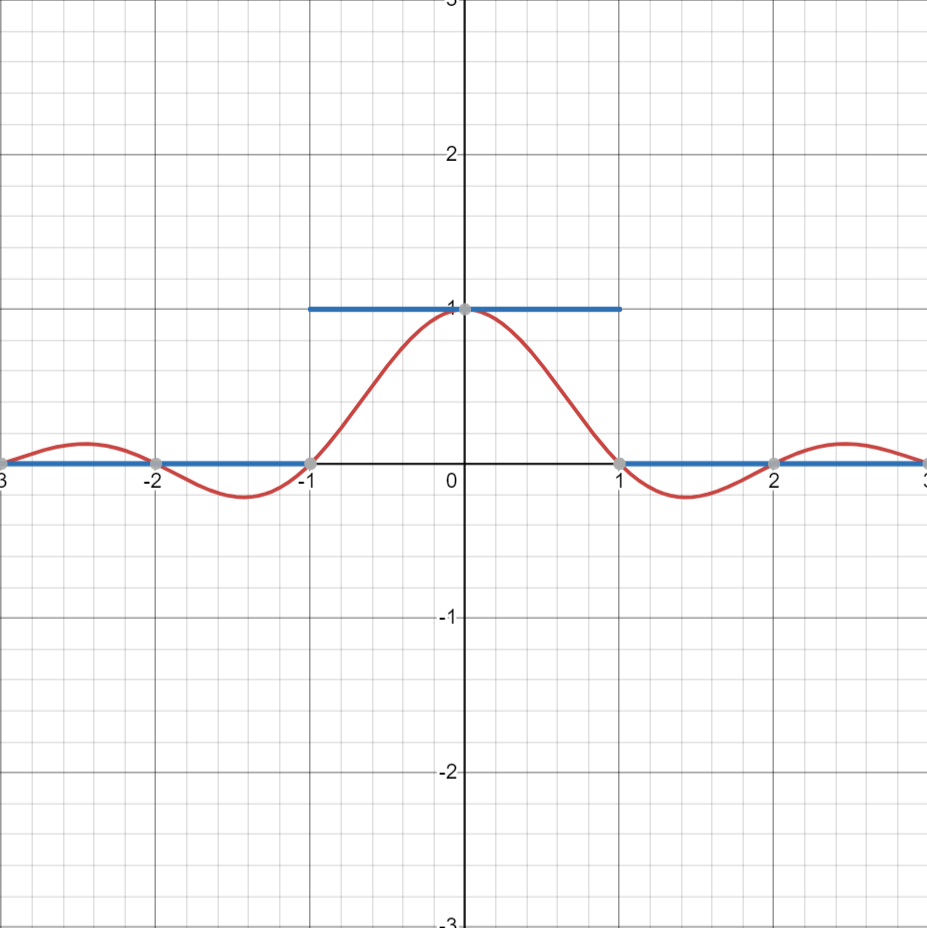
\includegraphics[width=0.5\linewidth]{pictures/image for Q3.png}
    \caption{graph of $f(x)$(purple) and $\hat{f}(\xi)$(green) in Q3}
    \label{fig:enter-label}
\end{figure}


\item Assume $f$ is a real-valued function of a real variable $x$.  Assume $f$ is even.  Show that $\hat{f}$ is real-valued.  
\textbf{Solution:}
\\
\[
\text{let } f(x), x \in\mathbb{R} \;\;\; \text{and $f(x)$ be even}
\]
\[
\hat{f}(\xi) = \int_{-\infty}^{\infty} f(x) e^{-2\pi i x \xi} \; dx 
\]
can be written as
\[
\hat{f}(\xi) = \int_{-\infty}^{\infty} f(x)\cos{(2\pi  x \xi)} - f(x)i\sin{(2\pi  x \xi)}\;dx
\]
\[
=\int_{-\infty}^{\infty} f(x)\cos{(2\pi  x \xi)}\;dx - \int_{-\infty}^{\infty}f(x)i\sin{(2\pi  x \xi)}\;dx
\]
since $f(x)$ is an even function and $sin(2\pi i x \xi)$ is an odd function, the product is odd
\\
\[
\therefore \; \int_{-\infty}^{\infty}f(x)i\sin{(2\pi  x \xi)}\;dx =0
\]
this integral evaluates to $0$ by symmetry and we are left with
\[
\int_{-\infty}^{\infty} f(x)\cos{(2\pi  x \xi)}\;dx
\]
and since $f(x)\cos{(2\pi  x \xi)}$ is even
\[
\int_{-\infty}^{\infty} f(x)\cos{(2\pi  x \xi)};dx = 2\int_{0}^{\infty} f(x)\cos{(2\pi  x \xi)}\;dx
\]
\[
\hat{f}(\xi)=2\int_{0}^{\infty} f(x)\cos{(2\pi  x \xi)}\;dx
\]
by observing the integral we see that the integral yields only real value, thus
\[
\hat{f}(\xi)\in\mathbb{R} \text{ if } f(x), x \in\mathbb{R} \;\;\; \text{and $f(x)$ be even}
\]
\newline




\item Find a fundamental set of solutions for the Euler equation 
\[
t^{2} y'' + 3t y' + 4y = 0, \;\;\; t> 0 
\]
\text{we can get the characteristic equation of this ODE to be}
\[
r^2+2r+4=0
\]
\[
(r+1)^2=-2
\]
\[
r=-1\pm i\sqrt{2}
\]
we will use the positive solution to proceed
\[
\text{let $\phi = t^{-1+i\sqrt{2}}$}
\]
we can rewrite it as
\[
\phi = e^{(-1+i\sqrt{2})\ln{t}}
\]
\[
=e^{(-\ln{t}+i\sqrt{2}\ln{t})}
\]
\[
=t^{-1}\cos{(\sqrt{2}\ln{t})}+t^{-1}i\sin{(\sqrt{2}\ln{t})}
\]
let $y_1=Re(\phi)$ and $y_2=Im(\phi)$
\[
y_1=t^{-1}\cos{(\sqrt{2}\ln{t})}
\]
\[
y_2=t^{-1}\sin{(\sqrt{2}\ln{t})}
\]
and the solution of this ODE is\[
y=c_1y_1 + c_2y_2 \;\;\; \text{where $c_1,c_2 \in \mathbb{R}$}
\]




\item Integrate 
\[
\int_{0}^{\pi} \exp((-1+i)t) \; dt
\]
and use this value to deduce values for the integrals 
\[
\int_{0}^{\pi} e^{-t} \cos t \; dt, \;\;\;  \int_{0}^{\pi} e^{-t} \sin t \; dt
\]
\text{Solution:}\\
we can first solve this integral in the exponential form as follows
\[
\int_{0}^{\pi} e^{(-1+i)t}\; dt = \frac{e^{(-1+i)t}}{-1+i} \left|_{t=0}^{t=\pi} \right.
\]
\[
= \frac{e^{(-1+i)\pi}}{-1+i}- \frac{1}{-1+i}
\]
\[
=\frac{e^{(-1+i)\pi} -1}{-1+i} = \frac{e^{-\pi}\cos{(\pi)}+ e^{-\pi}\sin{(\pi)} -1}{-1+i}
\]
\[
=\frac{-e^{-\pi} -1}{-1+i}
\]
we multiply the numerator and the denominator by the complex conjugate of the denominator
\[
=\frac{(-e^{-\pi} -1)(-1-i)}{2}=\frac{(e^{-\pi}+1)+i(e^{-\pi}+1)}{2}
\]
thus this integral evaluates to\[
\int_{0}^{\pi} e^{(-1+i)t}\; dt = \frac{e^{-\pi}+1}{2} + i\frac{e^{-\pi}+1}{2}
\]
let the solution be denoted by $z$, we have\[
Re(z)=Im(z)=\frac{e^{-\pi}+1}{2}
\]
to deduce the value of the 2 integrals provided, we use Euler's identity to rewrite the complex exponential
\[
\int_{0}^{\pi} e^{(-1+i)t}\; dt = \int_{0}^{\pi} e^{-t}e^{it}\; dt
\]
\[
=\int_{0}^{\pi} e^{-t}\cos{t} \; dt + i\int_{0}^{\pi} e^{-t}\sin{t} \; dt
\]
by observing the real and imaginary parts of the solution we obtained earlier, we can deduce that
\[
\int_{0}^{\pi} e^{-t}\cos{t} \; dt = Re(z) = \frac{e^{-\pi}+1}{2}
\]
\[
\int_{0}^{\pi} e^{-t}\sin{t} \; dt = Im(z)=  \frac{e^{-\pi}+1}{2}
\]







    
    \item \colorbox{yellow}{$\ast$}  Find 
    \[
    \int_{C} x \; dz
    \]
    where $C$ is the directed line segment from the origin to $1+i$.
    

\textbf{Solution:}
\\
to evaluate this integral, we first parameterize the path C as follows
\[
C:\; r(t) = t+it \;\; \{0\leq t\leq 1\}
\]
\[
r'(t)=1+i
\]
we notice that\[
x=y=t
\]
now we can evaluate the integral as follows
\[
\int_{0}^{1} f(r(t))r'(t)\; dt
\]
which gives us
\[
\int_{0}^{1} t(1+i) \; dt
\]
\[
=\int_{0}^{1} t+it \; dt = \left[\frac{1}{2}t^2 + i\frac{1}{2}t^2 \right ] \left|_{t=0}^{t=1} \right.
\]
\[
=\frac{1}{2}+i\frac{1}{2}
\]
Thus this integral evaluates to \[
\int_{C} x \; dz = \frac{1}{2}+i\frac{1}{2}
\]


\newline




\item Find 
\[
\int_{C} f(z) \; dz
\]
where $f(z) = y-x - 3ix^{2}$ where $C$ is the line from the origin to $i$ followed by the line from $i$ to $1+i$.  
\textbf{Solution:}\\
we would first parameterize the paths into two distinct sections as follows
\[
C_1: \; r_1(t)=it \;\; \{0\leq t \leq 1\}
\]
\[
C_2: \; r_2(t)=t+i \;\; \{0\leq t \leq 1\}
\]
we can identify that
\[
r_1: \;\; x=0 \;\; y=t
\]
\[
r_2: \;\; x=t \;\; y=1
\]
now we find the derivatives
\[
r_1'(t)=i \;\; \{0\leq t \leq 1\}
\]
\[
r_2'(t)=1 \;\; \{0\leq t \leq 1\}
\]
and we need to find the function $f(z)=y-x-3ix^2$ on path $C_1$ and $C_2$
\[
f(r_1(t))=t
\]
\[
f(r_2(t))=1-t-3it^2
\]
now evaluating $f(z)$ along path $C_1$, we have
\[
\int_{0}^{1} it \; dt = i\frac{1}{2}t^2\left|_{t=0}^{t=1} \right.=\frac{1}{2}i
\]
evaluating $f(z)$ along path $C_2$, we have
\[
\int_{0}^{1} 1-t-3it^2 \; dt = \left[ t-\frac{1}{2}t^2-it^3 \right]\left|_{t=0}^{t=1}  \right. = \frac{1}{2}-i
\]
now we take the sum of the two results to obtain
\[
\int_C f(z)\;dz = \int_{C_1} f(z)\;dz + \int_{C_2} f(z)\;dz = \frac{1}{2}-\frac{1}{2}i
\]






    \item  \colorbox{yellow}{$\ast$}  Use the Cauchy Integral Formula to find 
    \[
    \int_{C} \frac{1}{z^{2} -1} \; dz
    \]
    where $C$ is the circle centered at the origin with radius 2.  $C$ has the counter-clockwise orientation and $C$ is being traversed one time.  

\begin{remark}
Hint:  Partial fraction decomposition.  You do not have to simplify your final answer.        
\end{remark}
\textbf{Solution:}\\
first, we would rewrite the denominator of the integrand as follows
\[
\int_{C} \frac{1}{(z+1)(z-1)} \; dz
\]
and we notice that the integral has two singularities of multiplicity of one at $z=\pm 1$
\\
the positively oriented path $C$ enclosed both of the singularities
\\
to apply the Cauchy-Integral Formula
\[
\int_{C} \frac{f(x)}{z-z_0}=2\pi i f(z_0)
\]
we use partial fraction decomposition to break the integrand as follows 
\[
\frac{A}{z+1} + \frac{B}{z-1} = \frac{1}{(z+1)(z-1)}
\]
\[
A(z-1)+B(z+1)=1
\]
\[
\text{let }z=1, \;\; B=\frac{1}{2}
\]
\[
\text{let }z=-1, \;\; A=-\frac{1}{2}
\]
Thus the integral can be rewritten as
\[
\int_{C} \frac{1}{(z+1)(z-1)} \; dz = \frac{1}{2} \int_{C} \frac{1}{z-1} \; dz - \frac{1}{2} \int_{C} \frac{1}{z+1}\; dz
\]
applying the Cauchy Integral formula, we can see that this integral evaluates to
\[
\int_{C} \frac{1}{z^{2} -1} \; dz = \pi i - \pi i = 0
\]
\newline

    
 \item Use the Cauchy Integral Formula to find 
 \[
 \int_{C} \frac{ze^{z}}{z^{3} + i}
 \]
 Where $C$ is the circle centered at $-\frac{\sqrt{3}}{2} -  \frac{i}{2}$ with radius $\frac{1}{4}$. 

\begin{remark}
    You do not have to simplify your final answer.  
\end{remark}
\textbf{Solution:}\\
first, we would rewrite the denominator of the integrand as before
\[
\int_{C} \frac{ze^{z}}{z^{3} + i} = \int_{C} \frac{ze^{z}}{(z-i)(z^2+iz-1)}
\]
we have singularities at
\[
z=i
\]
\[
z^2+iz-1=0
\]
the quadratic equation can be solved as follows
\[
z^2+iz-1=(z+\frac{i}{2})^2-\frac{3}{4}=0
\]
\[
z+\frac{i}{2}=\pm \frac{\sqrt{3}}{2}
\]
\[
z=\pm \frac{\sqrt{3}}{2} - \frac{1}{2}i
\]
we can see that only $z=-\frac{\sqrt{3}}{2} - \frac{1}{2}i$ lies on our path of integration
\\
and with the information of the roots, we can rewrite the denominator further
\[
\int_{C} \frac{ze^{z}}{z^{3} + i} = \int_{C} \frac{ze^{z}}{(z-i)(z-z_1)(z-z_2)}
\]
\[
\text{where }z_1=\frac{\sqrt{3}}{2} - \frac{1}{2}i
\]
\[
z_2= -\frac{\sqrt{3}}{2} - \frac{1}{2}i
\]
we see that the only singularity involved along given path $C$ is $z_2$, thus we can identify that
\[
f(z)=\frac{ze^z}{(z-i)(z-z_1)}
\]
using the Cauchy Integral formula, we have
\[
 \int_{C} \frac{ze^{z}}{z^{3} + i} = 2\pi i f(z_2) =2\pi i \frac{z_2e^{z_2}}{(z_2-i)(z_2-z_1)}
\]
\[
\text{where }z_1=\frac{\sqrt{3}}{2} - \frac{1}{2}i \;\; z_2 = -\frac{\sqrt{3}}{2} - \frac{1}{2}i
\]


\end{enumerate}
\end{document}